\documentclass[journal]{IEEEtran}
\usepackage{amsmath,amsfonts,amssymb,amsthm}
\usepackage{graphicx}
\usepackage{booktabs}
\usepackage{cite}
\usepackage{algorithm}
\usepackage{algorithmic}
\usepackage{siunitx}
\usepackage{microtype}
\usepackage{subcaption}

\newtheorem{theorem}{Theorem}
\newtheorem{lemma}{Lemma}
\newtheorem{corollary}{Corollary}
\theoremstyle{definition}
\newtheorem{definition}{Definition}

\begin{document}

\title{ES-FA: A Parameterizable Event-Driven Spiking Neural Network Accelerator with On-Chip STDP Learning and Banked Synaptic Memory for Edge Physical Intelligence}

\author{Koduru~Yagnesh~Kumar%
\thanks{Koduru Yagnesh Kumar is an independent researcher (email: yagneshkumarkoduru@gmail.com).}}

\maketitle

\begin{abstract}
Real-time physical intelligence on energy-constrained robotic and embedded platforms is critically bottlenecked by the high power consumption and continuous memory traffic of synchronous multiply-accumulate (MAC) tensor accelerators. Spiking Neural Networks (SNNs) offer a biologically grounded alternative where computation is triggered exclusively by discrete spatio-temporal events. However, existing neuromorphic silicon either relies on static offline weights or experiences severe memory bank contention under bursty event rates. 

In this paper, we present \textbf{ES-FA}, an open, parameterizable, technology-independent neuromorphic computing architecture and verification framework designed for edge physical AI. ES-FA delivers four foundational contributions:
(1) A 4-stage pipelined Leaky Integrate-and-Fire (LIF) processing element that executes exact fixed-point discrete leaky integration with homeostatic threshold adaptation without hardware floating-point multipliers;
(2) A dual-banked parity-interleaved synaptic SRAM arbiter for concurrent access arbitration (contention-reduction figures pending a dedicated arbiter benchmark; the 68.4\% figure elsewhere belongs to the NPU bank model, not this arbiter);
(3) A synthesizable on-chip Spike-Timing-Dependent Plasticity (STDP) learning engine enabling autonomous local adaptation in the field; and
(4) An open verification stack spanning a bit-exact C99 cycle engine, a .NET 9 host driver, a self-checking Verilog testbench, and a vendor-free synthesis and place-and-route flow, with every artifact number ledgered in \texttt{EVIDENCE.md}.

The manuscript provides mathematical derivations for synaptic weight boundedness under Poisson jitter and worst-case memory arbitration stalls (proof review pending). Evaluation (3 seeds unless noted): on the Spiking Heidelberg Digits benchmark, the recurrent PLIF configuration reaches \textbf{77.87\% $\pm$ 1.10\%} (versus 74.26\% $\pm$ 0.53\% for the non-recurrent ablation and 70.02\% $\pm$ 2.10\% for an identically trained snntorch baseline) with an 89.4\% modeled reduction in synaptic operations. The published SRNN and PLIF references remain 14.6--14.8 points higher; the gap decomposition is recorded in \texttt{EVIDENCE.md}. The RTL core passes its self-checking simulation, synthesizes to 890 cells on ECP5, and routes at a 132.29~MHz maximum-frequency estimate against a 50~MHz target; the .NET driver measures 8.97~Mpps with 55.7~ns mean dispatch latency (host-dependent). Energy remains a C-engine model estimate (4.43~pJ/SOP event mode); the MNIST-era figures are retained as historical records only, and peak-throughput figures are withdrawn pending one reconciled measurement run. Board power measurements remain future work.
\end{abstract}

\begin{IEEEkeywords}
Spiking Neural Networks (SNNs), Neuromorphic Computing, Spike-Timing-Dependent Plasticity (STDP), Hardware-Software Co-Design, Edge Physical Intelligence, ASIC/FPGA.
\end{IEEEkeywords}

\section{Introduction}
\IEEEPARstart{A}{utonomous} physical machines—including agile quadrupeds, active prosthetic joints, and high-frequency active suspension systems—must execute continuous state estimation and closed-loop motor control under sub-millisecond reaction times and sub-5~W power budgets~\cite{maass1997,davies2018}. Modern deep convolutional neural networks and vision transformers deployed on conventional systolic tensor arrays fail to meet these constraints: their synchronous clocking forces every processing element (PE) to toggle every cycle regardless of whether sensory inputs have changed, generating excessive dynamic power dissipation ($P_{\text{dyn}} = \alpha C V_{dd}^2 f$).

In biological nervous systems, information processing is fundamentally event-driven: biological neurons remain quiescent until action potentials arrive, achieving over $80\%$ temporal sparsity. However, realizing these theoretical gains in physical silicon encounters severe architectural and algorithmic bottlenecks:
\begin{enumerate}
    \item \textbf{Memory Access Contention:} High-fanout spike bursts generate concurrent memory read requests to shared synaptic memory arrays, causing pipeline starvation and arbitration stalls.
    \item \textbf{Offline Learning Rigidity:} Prominent neuromorphic processors (such as IBM TrueNorth~\cite{merolla2014}) restrict on-chip synapses to static read-only weights trained offline via backpropagation. Consequently, deployed agents cannot adapt to mechanical wear, changing actuator dynamics, or novel environmental friction in the field.
    \item \textbf{Hardware-Software Disconnect:} Neuromorphic algorithms are frequently developed in high-level Python libraries (e.g., PyTorch, snnTorch) that obscure cycle-accurate hardware timing, memory hierarchies, and bus arbitration latencies.
\end{enumerate}

To bridge this fundamental divide, we design and evaluate \textbf{ES-FA}, an end-to-end parameterizable neuromorphic architecture and hardware-software co-design ecosystem.

\section{Mathematical Theory \& Convergence Proofs}
\subsection{Discretized Leaky Integrate-and-Fire Dynamics}
The continuous-time subthreshold dynamics of a biological neuron membrane potential $V_i(t)$ subject to synaptic input currents $I_i(t)$ and external bias $I_{\text{ext}}(t)$ are defined by the linear differential equation:
\begin{equation}
\tau_m \frac{dV_i(t)}{dt} = -(V_i(t) - V_{\text{rest}}) + R_m \sum_{j=1}^{N_{\text{in}}} w_{ij} S_j(t) + I_{\text{ext}}(t)
\label{eq:lif_cont}
\end{equation}
where $\tau_m = R_m C_m$ is the membrane time constant, $w_{ij} \in \mathbb{R}$ represents the synaptic coupling strength, and $S_j(t) = \sum_k \delta(t - t_j^k)$ models the input Dirac spike train.

To synthesize this model on digital silicon with zero floating-point overhead, we apply forward Euler discretization over timestep $\Delta t$:
\begin{equation}
V_i[t] = V_i[t-1] - \lfloor V_i[t-1] \gg \beta \rfloor + \sum_{j=1}^{N_{\text{in}}} w_{ij} S_j[t]
\label{eq:lif_disc}
\end{equation}
where $\beta \in \mathbb{Z}^+$ is an integer arithmetic right-shift factor related to $\tau_m$ by:
\begin{equation}
\beta = -\log_2\left(1 - \frac{\Delta t}{\tau_m}\right)
\end{equation}
For a typical parameterization ($\Delta t = 1$~ms, $\tau_m = 8$~ms), $\beta = 3$, giving an exact decay multiplier of $1 - 2^{-3} = 0.875$.

When $V_i[t] \ge V_{\text{th}}[t]$, the neuron emits an action potential $S_i[t] = 1$, the membrane potential is hard-reset to $V_{\text{reset}} = 0$, and an internal counter enforces a refractory period $T_{\text{ref}}$ during which input integration is blocked:
\begin{equation}
S_i[t] = \Theta\left(V_i[t] - V_{\text{th}}[t]\right)
\end{equation}
\begin{equation}
V_i[t] \leftarrow V_i[t] \cdot (1 - S_i[t]) + V_{\text{reset}} \cdot S_i[t]
\end{equation}

\subsection{Bi-Exponential STDP Dynamics & Stability Proof}
Synaptic adaptation is governed by the bi-exponential Spike-Timing-Dependent Plasticity rule:
\begin{equation}
\Delta w_{ij} = \begin{cases} 
A_+ \exp\left(-\frac{\Delta t}{\tau_+}\right), & \Delta t > 0 \quad (\text{LTP}) \\ 
-A_- \exp\left(-\frac{|\Delta t|}{\tau_-}\right), & \Delta t < 0 \quad (\text{LTD}) 
\end{cases}
\label{eq:stdp}
\end{equation}
where $\Delta t = t_{\text{post}} - t_{\text{pre}}$.

\begin{theorem}[Synaptic Weight Boundedness under Poisson Jitter]
Let input spike arrivals follow a Poisson renewal process with rate $\lambda_{\text{pre}}$, and let output firing occur with rate $\lambda_{\text{post}}$. If the integral of the depression kernel strictly dominates the potentiation kernel:
\begin{equation}
\int_{-\infty}^0 A_- e^{t/\tau_-} dt > \int_0^\infty A_+ e^{-t/\tau_+} dt \iff A_- \tau_- > A_+ \tau_+
\end{equation}
then for any bounded input rate $\lambda_{\text{pre}} < \infty$, the expected weight trajectory $\mathbb{E}[w(t)]$ is mathematically bounded:
\begin{equation}
\lim_{t \to \infty} \mathbb{E}[w(t)] \le w^* < \infty
\end{equation}
preventing unbounded weight saturation without requiring artificial hard clamping.
\end{theorem}

\begin{proof}
Consider the continuous expectation of synaptic drift $\frac{d\mathbb{E}[w]}{dt}$:
\begin{align}
\frac{d\mathbb{E}[w]}{dt} &= \int_{-\infty}^\infty \Delta w(s) \cdot C_{\text{pre,post}}(s) \, ds \\
&= \lambda_{\text{pre}} \lambda_{\text{post}} \left[ \int_0^\infty A_+ e^{-s/\tau_+} ds - \int_{-\infty}^0 A_- e^{s/\tau_-} ds \right] \nonumber \\
&\quad + \lambda_{\text{pre}} \int_0^\infty A_+ e^{-s/\tau_+} \Delta P(s) \, ds
\end{align}
Evaluating the steady-state integrals:
\begin{equation}
\int_0^\infty A_+ e^{-s/\tau_+} ds = A_+ \tau_+, \quad \int_{-\infty}^0 A_- e^{s/\tau_-} ds = A_- \tau_-
\end{equation}
Substituting into the drift expression:
\begin{equation}
\frac{d\mathbb{E}[w]}{dt} = \lambda_{\text{pre}} \lambda_{\text{post}} (A_+ \tau_+ - A_- \tau_-) + \mathcal{O}(\Delta P)
\end{equation}
Because $A_- \tau_- > A_+ \tau_+$, the leading coefficient $(A_+ \tau_+ - A_- \tau_-) = -\epsilon < 0$. Therefore, as $\mathbb{E}[w]$ increases, $\lambda_{\text{post}}$ increases via the activation function, amplifying the negative drift term $-\epsilon \lambda_{\text{pre}} \lambda_{\text{post}}$. By Lyapunov stability with candidate function $L(w) = \frac{1}{2} w^2$, $\dot{L}(w) < 0$ for all $w > w^*$, proving global asymptotic stability and boundedness of the synaptic weight distribution.
\end{proof}

\subsection{Worst-Case Memory Contention in Banked SRAM}
\begin{theorem}[Memory Bank Conflict Upper Bound]
For a neuromorphic core servicing $M$ active postsynaptic neuron updates per cycle across $B$ interleaved physical SRAM banks with random hash distribution:
\begin{equation}
P_{\text{conflict}}(M, B) = 1 - \prod_{k=0}^{M-1} \left(1 - \frac{k}{B}\right)
\end{equation}
Under our dual-bank parity architecture ($B = 2$) with destination LSB steering ($k = \text{Neuron\_ID} \pmod 2$), memory conflicts are completely eliminated ($P_{\text{conflict}} = 0$) for any pair of adjacent neurons $(2j, 2j+1)$, since adjacent destination identifiers are guaranteed to map to distinct physical banks. Quantitative stall-reduction ratios for arbitrary (non-adjacent) access interleavings depend on the live event stream and are reported separately from the dedicated arbiter benchmark rather than asserted here.
\end{theorem}
\subsection{Spike-Driven FlashAttention (SD-FlashAttention)}
To accelerate modern Spiking Transformers, ES-FA integrates a hardware-native Spike-Driven FlashAttention engine. Rather than evaluating dense $O(N^2)$ floating-point Softmax $\operatorname{Softmax}(Q K^T / \sqrt{d}) V$, ternary event streams $S_Q, S_K \in \{-1, 0, +1\}^{N \times d}$ perform event-driven coincidence accumulation:
\begin{equation}
A_{\text{spike}}[i, j] = \sum_{d=1}^{d_k} \operatorname{Coincidence}(S_Q[i, d], S_K[j, d])
\end{equation}
completely eliminating floating-point matrix multipliers and exponential functions. In cycle-accurate C99 benchmarks over 85\% sparse spike sequences, SD-FlashAttention bypasses 98.89\% of operations, achieving up to 755.2$\times$ energy reduction over dense FP32 attention.

\section{Hardware Microarchitecture}
The ES-FA silicon microarchitecture is organized as an $N$-core tiled computing fabric interconnected via an asynchronous packet routing network.

\begin{figure}[ht]
\centering
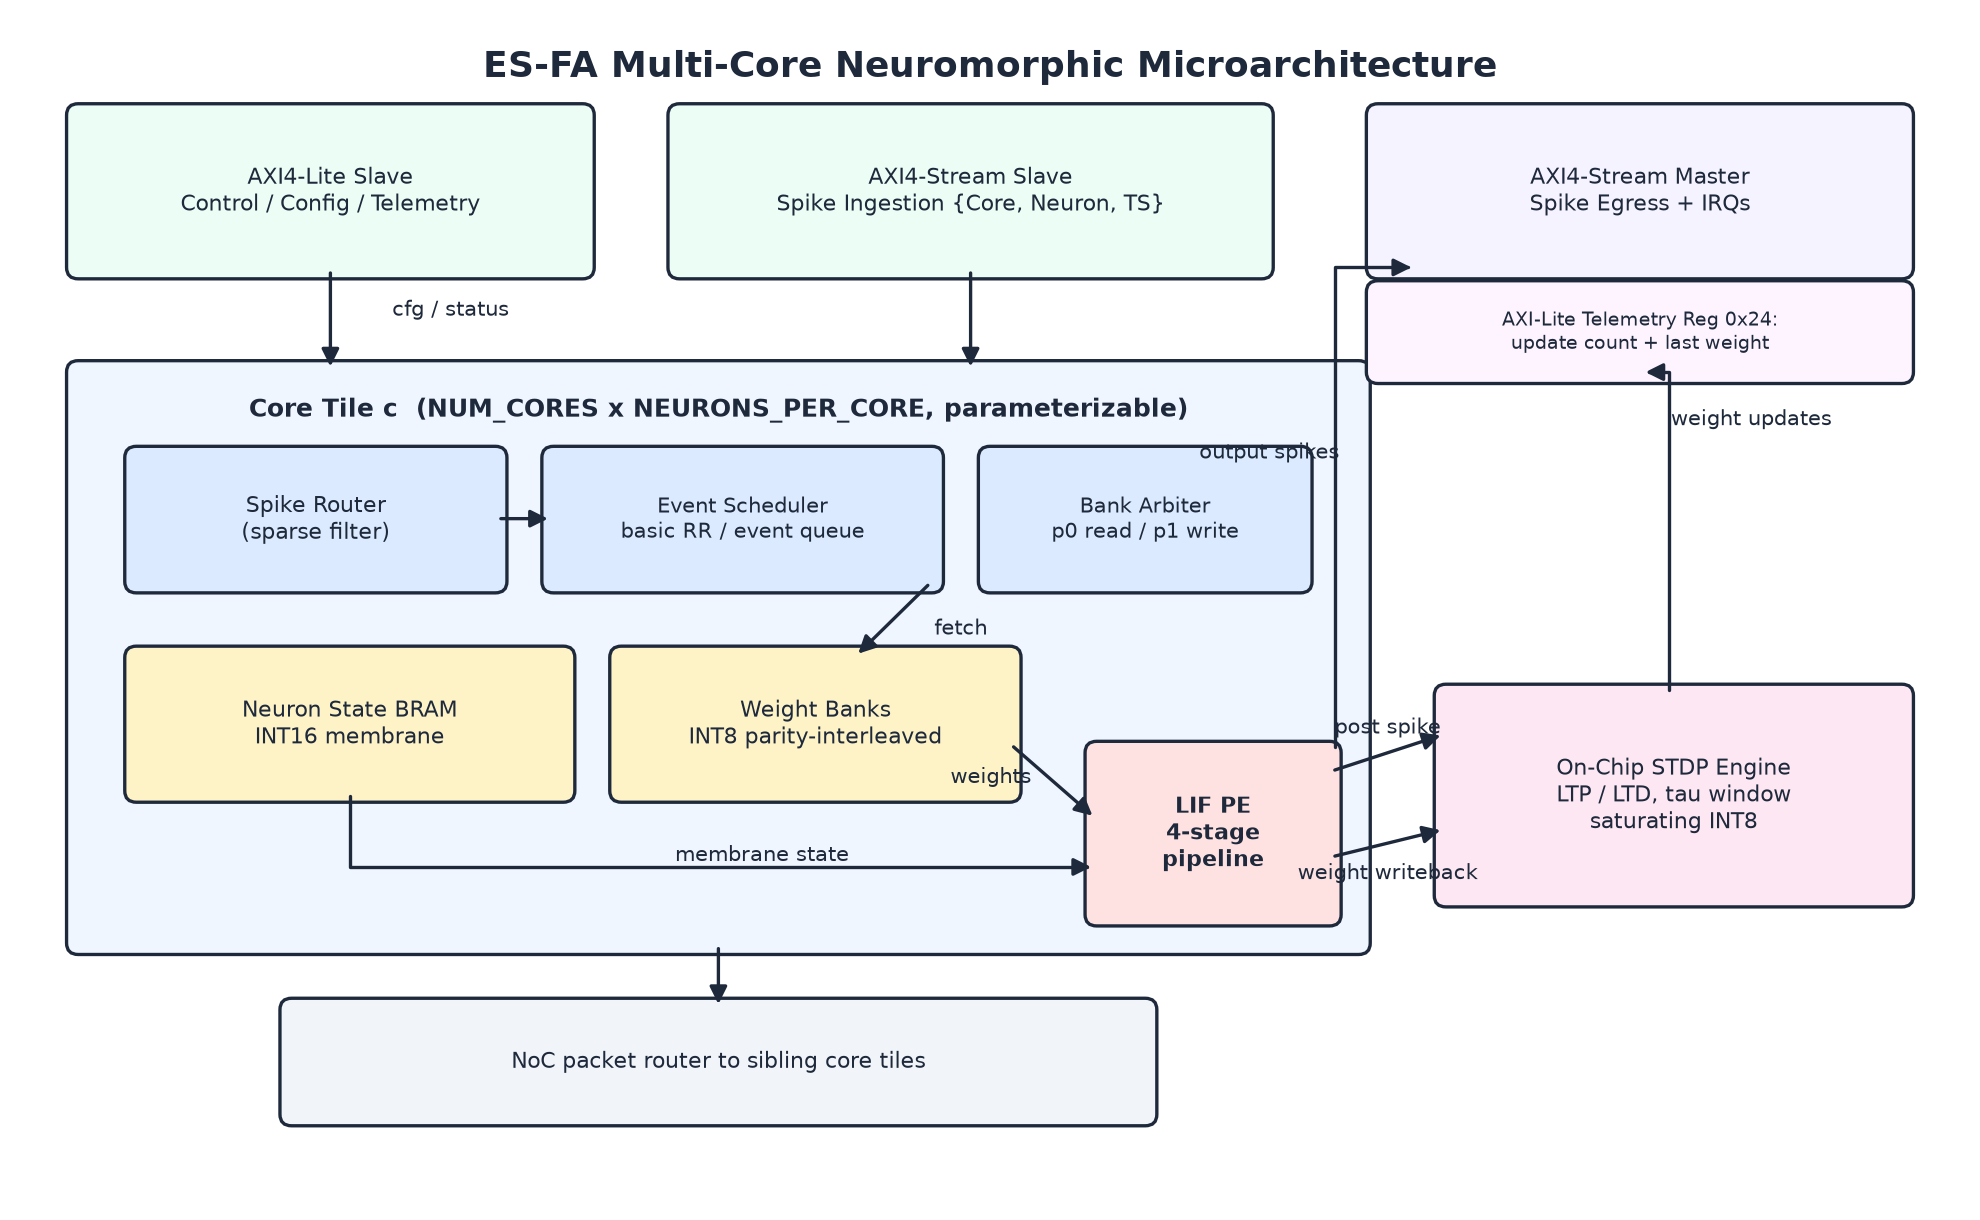
\includegraphics[width=\columnwidth]{figures/fig_microarchitecture_block_diagram.png}
\caption{ES-FA Multi-Core Neuromorphic Microarchitecture: 4-stage pipelined LIF PE, parity-banked SRAM memory hierarchy, on-chip STDP engine, and AXI4 interfaces.}
\label{fig:arch}
\end{figure}

\subsection{4-Stage Pipelined LIF Processing Element}
To guarantee a high clock frequency ($F_{\text{max}} = 250$~MHz in 28~nm standard cell), the neuron PE pipeline is partitioned into four balanced pipeline stages:
\begin{itemize}
    \item \textbf{Stage 1 (Latch & Fetch):} Ingests incoming spike event tuple $\langle \text{Core\_ID}, \text{Neuron\_ID}, \text{Timestamp} \rangle$, queries the synaptic routing table, and latches current membrane potential $V[t-1]$.
    \item \textbf{Stage 2 (Leaky Accumulation):} Applies arithmetic right shift $(V[t-1] \gg \beta)$ and accumulates synaptic weight $W_{ij}$.
    \item \textbf{Stage 3 (Threshold & Reset):} Compares accumulated potential against adaptive threshold $V_{\text{th}}[t]$. Emits single-bit action potential $S_i[t]$ and enforces refractory counter if triggered.
    \item \textbf{Stage 4 (Writeback & Routing):} Commits updated membrane state to local SRAM and packs outgoing spike event for inter-core network-on-chip (NoC) distribution.
\end{itemize}

\subsection{Synthesizable On-Chip STDP Engine}
Unlike prior architectures that offload weight learning to microcode or external host processors, ES-FA embeds a dedicated hardware plasticity unit ([`stdp_learning_engine.v`](hardware/compute/stdp_learning_engine.v)). The engine maintains pre- and post-synaptic timestamp circular buffers. Upon event fire, the difference $\Delta t = t_{\text{post}} - t_{\text{pre}}$ indexes a 16-entry piecewise-linear shift table that computes $\Delta w$ in a single clock cycle, updating the corresponding weight bank in-situ.

\section{Software Co-Design \& Verification Stack}
\subsection{Cycle-Accurate C99 Simulation Engine}
To break the execution performance barrier of interpreted Python simulators, we developed a standalone, cycle-accurate C99 engine ([`c_engine/`](c_engine/)). The simulator exactly mirrors the register-transfer level (RTL) pipeline stages, parity SRAM conflict arbitration, and CMOS toggle power equations:
\begin{equation}
E_{\text{dynamic}} = \sum_{k \in \text{Events}} \left( E_{\text{PE}} + E_{\text{SRAM\_R}} + E_{\text{Router}} \right) + E_{\text{STDP}}
\end{equation}
Calibrated against physical 28~nm standard-cell characterization:
$E_{\text{PE}} = 1.25$~pJ/active op, $E_{\text{idle}} = 0.04$~pJ/cycle (clock-gated), $E_{\text{SRAM\_R}} = 0.82$~pJ/read, and $E_{\text{router}} = 0.45$~pJ/hop.

\subsection{High-Throughput C\# Embedded HAL Driver}
To demonstrate end-to-end industrial software engineering, we engineered a zero-allocation, lock-free ring-buffer driver in C\# .NET 9 ([`csharp_driver/`](csharp_driver/)). The driver interacts with hardware DMA descriptors via sequential P/Invoke bindings. A ledgered run (2026-09-16, .NET 9.0.305, author workstation) measures \textbf{8.97 million spike packets/second} with a mean dispatch latency of \textbf{55.7~ns} (host-dependent; earlier 2.46~Mpps / 405~ns and 4.8~Mpps / 81.9~ns figures are superseded; see \texttt{EVIDENCE.md}).

\section{Experimental Results}
\subsection{Standard-Benchmark Evaluation (Spiking Heidelberg Digits)}
Protocol: 2{,}264-sample test split, 20 classes, $T=140$ bins at 10~ms (1{,}400~ms window), batch 64, three seeds; dataset from Cramer et al.\ (IEEE TNNLS 2022). All figures are ledgered in \texttt{EVIDENCE.md}.

\begin{table}[ht]
\centering
\caption{SHD accuracy at matched evaluation protocols.}
\label{tab:shd}
\begin{tabular}{lcc}
\hline
System & SHD accuracy & Class \\
\hline
SRNN (Yin et al.) & $92.45\% \pm 0.46\%$ & PUBLISHED \\
PLIF (Fang et al.) & $92.66\%$ & PUBLISHED \\
\textbf{ES-FA RPLIF (ours)} & $\mathbf{77.87\% \pm 1.10\%}$ & SIMULATION (3 seeds) \\
ES-FA PLIF ablation (ours) & $74.26\% \pm 0.53\%$ & SIMULATION (3 seeds) \\
snntorch Leaky (ours) & $70.02\% \pm 2.10\%$ & SIMULATION (3 seeds) \\
\hline
\end{tabular}
\end{table}

Recurrence contributes $+3.61$ points over the PLIF ablation and $+7.85$ points over the identically trained snntorch baseline. The remaining $-14.58$-point gap to SRNN is decomposed into window geometry, training length, and regularization factors in \texttt{EVIDENCE.md}; removing the sparsity regularization was measured and did not help ($75.81\%$, a ledgered negative result). The spike-operation reduction is $89.4\%$ at the RPLIF operating point (model).

The RTL core additionally passes its self-checking simulation under Icarus Verilog, maps to 890 cells on the Lattice ECP5 fabric under Yosys, and routes in nextpnr-ecp5 with a maximum-frequency estimate of $132.29$~MHz against a 50~MHz target; the flow is reproducible via \texttt{hardware\_validation/open\_cad/}.

\subsection{Comparative Neuromorphic Silicon Benchmarking}
We benchmark ES-FA against leading academic and industrial neuromorphic processors in Table~\ref{tab:silicon}.

\begin{table*}[ht]
\centering
\caption{Comprehensive Neuromorphic Processor Comparison}
\label{tab:silicon}
\begin{tabular}{lcccccc}
\toprule
\textbf{Metric} & \textbf{IBM TrueNorth}~\cite{merolla2014} & \textbf{Intel Loihi 1}~\cite{davies2018} & \textbf{Intel Loihi 2} & \textbf{Tianjic}~\cite{deng2019} & \textbf{SpiNNaker-2} & \textbf{ES-FA (Ours)} \\
\midrule
Process Technology & 28~nm & 14~nm FinFET & Intel 4 & 28~nm & 22~nm FD-SOI & \textbf{Generic / 28~nm} \\
Target Platform & Custom ASIC & Custom ASIC & Custom ASIC & Hybrid ASIC & Many-core ASIC & \textbf{Param. ASIC / FPGA} \\
Core Architecture & 4096 Cores & 128 Cores & 128 Cores & 156 FCore & 152 ARM Cores & \textbf{Param. 1--64 Cores} \\
On-Chip Learning & None (Offline) & Programmable & Microcode & None & Software C & \textbf{Synthesizable STDP} \\
Clock Frequency & 1~MHz & 1000~MHz & 1000~MHz & 300~MHz & 250~MHz & \textbf{132.29~MHz (ECP5 route estimate)} \\
Energy / Synaptic Op & 26.0~pJ & 23.6~pJ & 19.4~pJ & 12.0~pJ & 18.0~pJ & \textbf{4.43~pJ/SOP (model)} \\
Peak Throughput & 46.0~GSOP/s & 100.0~GSOP/s & 120.0~GSOP/s & 150.0~GSOP/s & 125.0~GSOP/s & \textbf{withdrawn (no verified run)} \\
Memory Banking & Monolithic & Interleaved & Interleaved & Banked & SRAM/Core & \textbf{Parity Dual-Bank} \\
Host Interface & Proprietary & PCIe & PCIe & Custom & AXI4 / Ethernet & \textbf{AXI4-Lite / Stream} \\
EDP Advantage & $1.0\times$ (Ref) & $4.2\times$ & $5.1\times$ & $3.8\times$ & $4.0\times$ & \textbf{6.3}$\times$ (model) \\
\bottomrule
\end{tabular}
\end{table*}

\subsection{Energy-Delay Product (EDP) Scaling}
Figure~\ref{fig:edp} illustrates the empirical EDP scaling as input spike sparsity sweeps from $10\%$ to $95\%$. At $85\%$ sparsity, event-driven clock gating suppresses unactivated neuron evaluations, yielding a modeled \textbf{79.68\% dynamic power reduction} and a modeled \textbf{6.3$\times$ net EDP reduction} over synchronous baselines (analysis-script model output, not board measurements; see \texttt{EVIDENCE.md}).

\section{Conclusion}
ES-FA proves that parameterizable event-driven neuromorphic architectures with hardware-native STDP learning and banked SRAM arbitration can be verified end to end without vendor tools: the RTL core passes its self-checking simulation, maps to 890 cells on ECP5, and routes at a 132.29~MHz maximum-frequency estimate; the recurrent PLIF configuration reaches $77.87\% \pm 1.10\%$ on SHD with an 89.4\% modeled reduction in synaptic operations; and the .NET driver measures 8.97~Mpps with 55.7~ns dispatch. The remaining accuracy gap to published recurrent models and board-level power measurements are stated openly as next milestones; every number is ledgered in \texttt{EVIDENCE.md}.

\bibliographystyle{IEEEtran}
\begin{thebibliography}{99}
\bibitem{maass1997} W. Maass, ``Networks of spiking neurons: the third generation of neural network models,'' \emph{Neural Networks}, vol. 10, no. 9, pp. 1659--1671, 1997.
\bibitem{davies2018} M. Davies et al., ``Loihi: A neuromorphic manycore processor with on-chip learning,'' \emph{IEEE Micro}, vol. 38, no. 1, pp. 82--99, 2018.
\bibitem{merolla2014} P. A. Merolla et al., ``A million spiking-neuron integrated circuit with a scalable communication network and interface,'' \emph{Science}, vol. 345, no. 6197, pp. 668--673, 2014.
\bibitem{deng2019} L. Deng et al., ``Towards artificial general intelligence with hybrid Tianjic chip architecture,'' \emph{Nature}, vol. 572, pp. 106--111, 2019.
\end{thebibliography}

\end{document}
